\chapter{Introduction and data}\label{chap:common}
\section{Introduction}\label{sec:intro}
The project concerns a client's existing generation assets and the investment
and operating decisions that can increase their value \cite{brief}. We study
batteries and electrolysers in Tier 1 and select Tier 2B to examine chronological
operation when future conditions must be predicted.

Our initial audit identified synchronised zero-generation records, missing
dates, midnight snapshots used as daily means, abnormally low demand records
and zero-volume price placeholders. The repair methods are full-day upstream
reaggregation, short-gap interpolation, calibrated cross-source reconstruction
and flagged whole-day imputation. These methods are distinguished in the
data audit rather than treated as a single class of replacement.

Tier 1 combines research on electricity trading, batteries, electrolysers and
financial conversion with mixed-integer linear programming. We compare
allocation among direct electricity sale, storage and hydrogen by economic
value with a policy that first sells all electricity for which current
demand exists. Gain means additional receipts less fixed operation and
annualised capital and renewals, against no investment under the same rule.
With assumed hydrogen net receipts (after non-electricity variable costs) of
\gbp\Netback/kg in 2020 pounds, a buyer accepting at most 10 tonnes per day and a 5\% real
discount rate, a common 20 MW electrolyser without batteries gives a mean
annual equivalent gain of \gbp\MeanA m under free allocation over 2020--25.
Contract thresholds, alternative dispatch rights, individual years and
battery chronology are then examined.

Tier 2B adds forecasts of generation, demand and prices to a rolling-horizon
operating model. It repeatedly plans several days ahead, executes only the
current day's decision and transfers the resulting battery stock to the next
day. Figure~\ref{fig:architecture} shows the data, investment, prediction and
state-feedback connections. Forecast accuracy and realised operating value
will be evaluated separately; the experimental protocol is specified in
Chapter~\ref{chap:tier2}.

\begin{figure}[H]
\centering
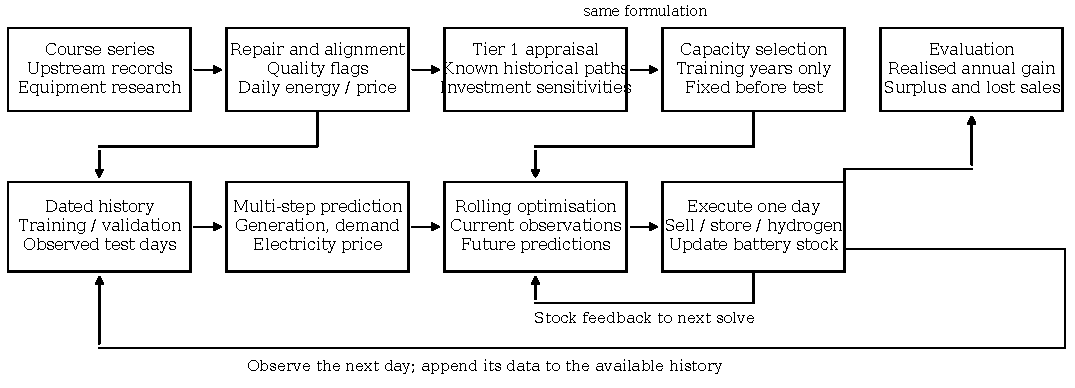
\includegraphics[width=\linewidth]{figures/model_architecture.pdf}
\caption{Study architecture. Tier 1 uses known historical paths. Tier 2B uses
past observations for forecasting and carries physical storage state forward;
its investment decision precedes the test period.}
\label{fig:architecture}
\end{figure}

\section{Data audit and reconstruction}\label{sec:data}
The five supplied files contain fuel-level generation, its total, simulated
wind-farm generation, demand and market index prices. The fuel total is
checked against its components; it is not added to them again. The separate
simulated farm is added to that total as the declared asset boundary.
Generation and demand are daily mean powers in MW, converted to MWh by
multiplying by 24. We retain 1 January 2020--17 September 2026: 2,452 days
in Coordinated Universal Time (UTC). Source checks use Elexon records and
National Energy System Operator (NESO) series.

\begin{table}[H]
\centering\small
\caption{Detected problems, evidence and repair. Date counts can overlap.}
\begin{tabularx}{\linewidth}{@{}P{.27\linewidth}Y@{}}
\toprule
Problem and extent & Identification and reconstruction \\
\midrule
Eight non-wind/solar fuels zero on 107 days; solar zero on 42 days &
Synchronous zeros conflict with archived records. Reaggregate Elexon actual
generation by production type; use calibrated fuel half-hour or NESO solar
series when that source is incomplete. Interpolate short gaps. \\
Midnight query endpoints: 7 generation, 350 demand, 346 price dates &
Original values reproduce the first timestamp rather than the full day.
Retrieve the complete UTC day and recalculate its mean. \\
Missing dates: 30 generation, 1 demand, 30 price &
Calendar gaps are verified against the dated upstream series. Restore those
records where available; otherwise use flagged whole-day estimates. \\
Invalid demand slots &
Some five-minute records are below 10,000 MW, including 636 MW on 2 August
2022. Retain valid slots and reconstruct others
from calibrated NESO demand; flag whole-day estimates. \\
Zero-volume price placeholders &
115,571 provider records have no traded volume. Exclude those placeholders,
volume-weight active providers within each half-hour, then average the day.
Retain genuine zero and negative prices. \\
\bottomrule
\end{tabularx}
\label{tab:repair}
\end{table}

The repaired files share a complete calendar; fuel components sum to total
generation, and the two price-unit columns retain their factor of 24.
The 2 August demand mean is reconstructed as 28,744 MW. The audit identifies
436 dates with interpolation or estimation, 323 with cross-source
reconstruction and 1,929 satisfying the strict quality flag; categories
overlap \cite{repair}. The full set supports the primary analysis; the strict
subset is a sensitivity check. All original values, replacements, source
records and quality flags are retained. Historical prices are converted
to 2020 pounds using monthly consumer price indices \cite{cpi}.

\section{Common notation and assumptions}\label{sec:global}
Only quantities shared by both tiers are defined here. Equipment decisions,
dispatch policies, forecast information and technical parameters are
introduced in their respective chapters.
\begin{table}[H]
\centering\small
\caption{Notation shared across the study.}
\begin{tabularx}{\linewidth}{@{}lY r@{}}
\toprule
Symbol & Meaning & Unit \\
\midrule
\(t\in\mathcal T\) & UTC day in the selected study period & day \\
\(G_t,D_t\) & Available generation and market demand (sales ceiling) & MWh \\
\(p_t\) & Market electricity price, in constant 2020 pounds & \gbp/MWh \\
\(S_t\) & Physical surplus, \(\max(G_t-D_t,0)\) & MWh \\
\(Y\) & Represented years: sum of each sampled day's calendar-year fraction & year \\
\bottomrule
\end{tabularx}
\end{table}
The supplied series describe a constructed system rather than observed
network congestion \cite{brief,teacher}. Existing generation is fixed;
its unchanged costs cancel in investment comparisons. Demand limits sales
and is not an additional unpaid internal load. We assume no electricity
imports, no additional export outlet and no payment for unused generation.
Spatial transfer limits are omitted. All monetary comparisons use constant
2020 pounds. These conventions are common to both tiers.
